\section{Triple Integrals} \label{S:11.7.Triple_Integrals}

\vspace*{-14 pt}
\framebox{\hspace*{3 pt}
\parbox{6.25 in}{\begin{goals}
\item How are a triple Riemann sum and the corresponding triple integral of a continuous function $f = f(x,y,z)$ defined?
\item What are two things the triple integral of a function can tell us?
\end{goals}} \hspace*{3 pt}}

\subsection*{Introduction}

We have now learned that we define the double integral of a continuous function $f = f(x,y)$ over a rectangle $R = [a,b] \times [c,d]$ as a limit of a double Riemann sum, and that these ideas parallel the single-variable integral of a function $g = g(x)$ on an interval $[a,b]$.   Moreover, this double integral has natural interpretations and applications, and can even be considered over non-rectangular regions, $D$.  For instance, given a continuous function $f$ over a region $D$, the average value of $f$, $f_{\mbox{\tiny{AVG}(D)}}$, is given by 
$$f_{\mbox{\tiny{AVG}(R)}} = \frac{1}{A(D)} \iint_D f(x,y) \, dA,$$
where $A(D)$ is the area of $D$.  Likewise, if $\delta(x,y)$ describes a mass density function on a lamina over $D$, the mass, $M$, of the lamina is given by 
$$M = \iint_D \delta(x,y) \, dA.$$ 

It is natural to wonder if it is possible to extend these ideas of double Riemann sums and double integrals for functions of two variables to triple Riemann sums and then triple integrals for functions of three variables. We begin investigating in Preview Activity \ref{PA:11.7}.

\begin{pa} \label{PA:11.7} Consider a solid piece granite in the shape of a box $B = \{(x,y,z) : 0 \leq x \leq 4, 0 \leq y \leq 6, 0 \leq z \leq 8\}$, whose density varies from point to point. Let $\delta(x, y, z)$ represent the mass density of the piece of granite at point $(x,y,z)$ in kilograms per cubic meter (so we are measuring $x$, $y$, and $z$ in meters). Our goal is to find the mass of this solid. 

Recall that if the density was constant, we could find the mass by multiplying the density and volume;  since the density varies from point to point, we will use the approach we did with two-variable lamina problems, and slice the solid into small pieces on which the density is roughly constant.

Partition the interval $[0,4]$ into 2 subintervals of equal length, the interval $[0,6]$ into 3 subintervals of equal length, and the interval $[0,8]$ into 2 subintervals of equal length. This partitions the box $B$ into sub-boxes as shown in Figure \ref{F:11.7.Box_domain}.
\begin{figure}[h]
\begin{center}
%\resizebox{!}{2.0in}{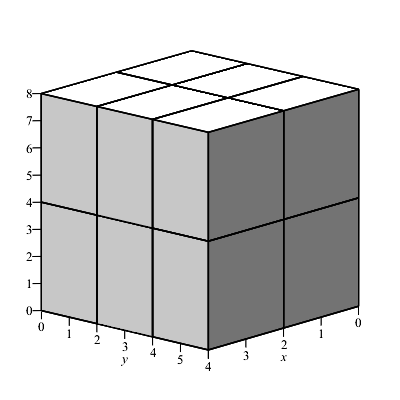
\includegraphics[trim=0cm 1cm 0cm 1cm, clip]{11_7_Box_domain}}
  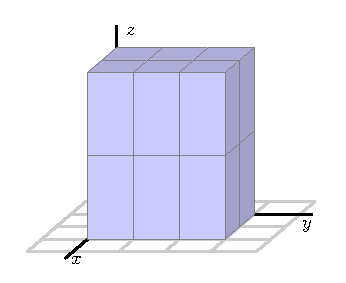
\includegraphics{figures/fig_11_7_preview.eps}
\end{center}
\caption{A partitioned three-dimensional domain.}
\label{F:11.7.Box_domain}
\end{figure}
%crop graphics in animate trim=<left> <bottom> <right> <top>, clip with includegraphics
    \ba
    \item Let $0=x_0 < x_1 < x_2=4$ be the endpoints of the subintervals of $[0,4]$ after partitioning. Draw a picture of Figure \ref{F:11.7.Box_domain} and label these endpoints on your drawing. Do likewise with $0=y_0 < y_1 < y_2 < y_3=6$ and $0=z_0 < z_1 < z_2=8$
    
    What is the length $\Delta x$ of each subinterval $[x_{i-1},x_i]$ for $i$ from 1 to 2?  the length of $\Delta y$?  of $\Delta z$?

	\item The partitions of the intervals $[0,4]$, $[0,6]$ and $[0,8]$ partition the box $B$ into sub-boxes. How many sub-boxes are there? What is volume $\Delta V$ of each sub-box?
	

	
	\item Let $B_{ijk}$ denote the sub-box $[x_{i-1},x_i] \times [y_{j-1},y_j] \times [z_{k-1}, z_k]$.
		%. Appropriately label each visible sub-box in your drawing of Figure \ref{F:11.7.Box_domain} according to this labeling scheme.
	Say that we choose a point $(x_{ijk}^*, y_{ijk}^*, z_{ijk}^*)$ in the $i,j,k$th sub-box for each possible combination of $i,j,k$.  What is the meaning of $\delta(x_{ijk}^*, y_{ijk}^*, z_{ijk}^*)$?  What physical quantity will $\delta(x_{ijk}^*, y_{ijk}^*, z_{ijk}^*) \Delta V$ approximate?
	

    \item What final step(s) would it take to determine the exact mass of the piece of granite?


\ea
\end{pa} 

\begin{activitySolution}

    \ba
    \item We have $x_0=0$, $x_1=2$, and $x_2=4$;  $y_0=0$, $y_1=2$, $y_2=4$, and $y_3=6$; and $z_0=0$, $z_1=4$, and $z_2=8$. This gives us $\Delta x = \frac{4-0}{2} = 2$, $\Delta y = \frac{6-0}{3} = 2$, and $\Delta z = \frac{8-0}{2} = 4$.  These points are labeled in figure below.

%\begin{figure}[h]
\begin{center}
\resizebox{!}{2.0in}{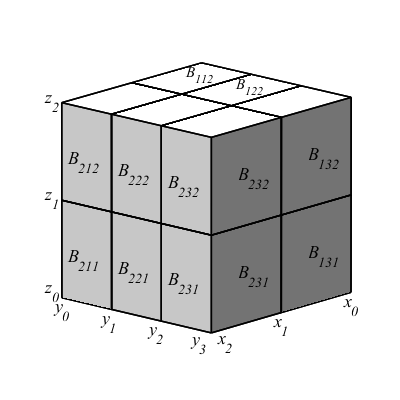
\includegraphics{figures/fig_11_7_Box_domain_PA_labeled.png}}
\end{center}
%\caption{A partitioned and labeled three-dimensional domain.}
%\label{F:11.7.Box_domain_PA_labeled}
%\end{figure}


	\item Since we partition the interval $[0,4]$ into 2 subintervals, the interval $[0,6]$ into 3 subintervals, and the interval $[0,8]$ into 2 subintervals, there are $(2)(3)(2) = 12$ sub-boxes of $B$.  Each sub-box has volume $\Delta x \ \Delta y \ \Delta z = (2)(2)(4) = 16$.

	
	\item The visible sub-boxes are labeled in the figure. Notice that we cannot see boxes
\[B_{111} = [x_0,x_1] \times [y_0, y_1] \times [z_0,z_1] \ \ \text{ and } \ \ B_{121} = [x_0,x_1] \times [y_1, y_2] \times [z_0,z_1].\]

If we consider the mass of the solid in sub-box $B_{ijk}$ as a constant $\delta(x_{ijk}^*, y_{ijk}^*, z_{ijk}^*)$ in kilograms per cubic meter, then the product $\delta(x_{ijk}^*, y_{ijk}^*, z_{ijk}^*) \Delta V$ will approximate the mass of the solid on sub-box $B_{ijk}$.


    \item To determine the mass of our solid, we sum the approximations of the masses on each sub-box and the take the limit as $\Delta x$, $\Delta y$, and $\Delta z$ go to 0. Thus, the mass of our solid is
\[\lim_{\substack{\Delta x \to 0 \\ \Delta y \to 0 \\ \Delta z \to 0}} \sum_{i=1}^m \sum_{j=1}^n \sum_{k=1}^l \delta(x_{ijk}^*, y_{ijk}^*, z_{ijk}^*) \Delta V.\]


\ea


\end{activitySolution}

\afterpa 

\subsection*{Triple Riemann Sums and Triple Integrals}

Through the application of a mass density distribution over a three-dimensional solid, Preview Activity \ref{PA:11.7} suggests that the generalization from double Riemann sums of functions of two variables to triple Riemann sums of functions of three variables is natural.  In the same way, so is the generalization from double integrals to triple integrals.  By simply adding a $z$-coordinate to our earlier work, we can define both a triple Riemann sum and the corresponding triple integral.

%Consider a solid box $B$ (like a box-shaped piece of granite as in Preview Activity \ref{PA:11.7}). Let $\delta(x, y, z)$ represent the density of solid at point $(x,y,z)$. To find the mass of this solid we use the integration process as we did in our Preview Activity. Defining triple Riemann sums and triple integrals involves keeping track of a lot of different objects, and we further develop our abilities to deal with these objects in our next activity.

%\begin{activity} \label{A:11.7.1} Suppose our box $B$ has the form $[a,b] \times [c,d] \times [r,s]$, that is $B = \{(x,y,z) : a \leq x \leq b, c \leq y \leq d, r \leq z \leq s\}$. We partition the box as illustrated in Figure \ref{F:11.7.Box_domain_2}.

\begin{figure}[ht]
\begin{center}
%\resizebox{!}{2.0in}{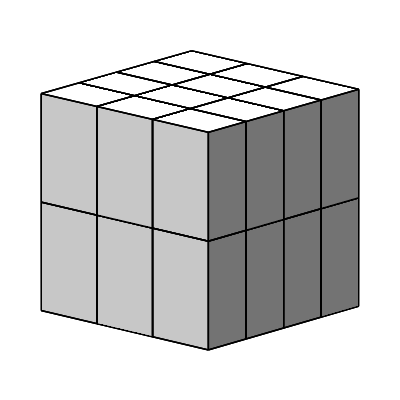
\includegraphics[trim=0cm 1.5cm 0cm 1.5cm, clip]{11_7_Box_domain_2}}
  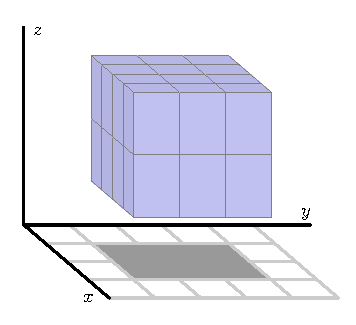
\includegraphics{figures/fig_11_7_partition.eps}
\end{center}
\caption{A partitioned three-dimensional domain.}
\label{F:11.7.Box_domain_2}
\end{figure}
%crop graphics in animate trim=<left> <bottom> <right> <top>, clip with includegraphics
	\ba
	\item Let $a=x_0 < x_1 < x_2 < x_3 < x_4=b$ be the endpoints of the subintervals of $[a,b]$ after partitioning. Label these endpoints in Figure \ref{F:11.7.Box_domain_2}. What is the length $\Delta x$ of each subinterval $[x_{i-1},x_i]$ for $i$ from 1 to 4? Your answer should be in terms of $a$ and $b$.
	
	
		
	\item Let $c=y_0 < y_1 < y_2 < y_3=d$ be the endpoints of the subintervals of $[c,d]$ after partitioning. Label these endpoints in Figure \ref{F:11.7.Box_domain_2}. What is the length $\Delta y$ of each subinterval $[y_{j-1},y_j]$ for $j$ from 1 to 3? Your answer should be in terms of $c$ and $d$.
	
	

	\item Let $r=z_0 < z_1 < z_2=s$ be the endpoints of the subintervals of $[r,s]$ after partitioning. Label these endpoints in Figure \ref{F:11.7.Box_domain_2}. What is the length $\Delta z$ of each subinterval $[z_{k-1},z_k]$ for $k$ from 1 to 2? Your answer should be in terms of $r$ and $s$.
	
	

	\item The partitions of the intervals $[a,b]$, $[c,d]$, and $[r,s]$ partition the box $B$ into sub-boxes. How many sub-boxes are there? What is the volume $\Delta V$ of each sub-box?
	
	
	
	\item Let $B_{ijk}$ denote the sub-box $[x_{i-1},x_i] \times [y_{j-1},y_j] \times [z_{k-1},z_k]$. Label each visible sub-box in Figure \ref{F:11.7.Box_domain_2}.
	
	
	
	
	\item Now let $(x_{ijk}^*, y_{ijk}^*, z_{ijk}^*)$ be an arbitrary point in the $i,j,k$th sub-box. Explain what the product
\[\delta(x_{ijk}^*, y_{ijk}^*, z_{ijk}^*) \Delta V\]
represents.



    \item If we were to add all the values $\delta(x_{ijk}^*, y_{ijk}^*, z_{ijk}^*) \Delta V$ for each $i$, $j$, and $k$, what does the resulting number approximate about the piece of granite?

	
	
	\item Write a triple sum using summation notation that expresses the arbitrary sum from part (k).
		
	
	\ea

\end{activity}
\begin{smallhint}

\end{smallhint}
\begin{bighint}

\end{bighint}
\begin{activitySolution}
	\ba
	\item The endpoints are labeled in the figure below. Since we are partitioning the interval $[a,b]$ into 4 subintervals of equal length, the length of each subinterval is $\Delta x = \frac{b-a}{4}$. 	
		
	\item The endpoints are labeled in the figure below. Since we are partitioning the interval $[c,d]$ into 3 subintervals of equal length, the length of each subinterval is $\Delta y = \frac{d-c}{3}$. 	

	\item The endpoints are labeled in the figure below. Since we are partitioning the interval $[r,s]$ into 2 subintervals of equal length, the length of each subinterval is $\Delta z = \frac{s-r}{2}$.

	\item The total number of sub-boxes is $4 \times 3 \times 2 = 24$. The volume of each sub-box is $\Delta V = \Delta x \ \Delta y \ \Delta z$. 
		
	\item The visible sub-boxes are shown in the figure below. 
	
	\item We are assuming a constant density of $\delta(x_{ijk}^*, y_{ijk}^*, z_{ijk}^*)$ in the sub-box $B_{ijk}$, so the product 
\[\delta(x_{ijk}^*, y_{ijk}^*, z_{ijk}^*) \Delta V\]
approximates the mass of the sub-box $B_{ijk}$.

    \item Since each $\delta(x_{ijk}^*, y_{ijk}^*, z_{ijk}^*) \Delta V$ approximates the mass of a sub-box, if we add all the values for each $i$, $j$, and $k$, the sum will approximate the mass of this piece of granite.
	
	\item A triple sum using summation notation that expresses the arbitrary sum from part (k) is
\[\sum_{k=1}^2 \sum_{j=1}^3 \sum_{i=1}^4 \delta(x_{ijk}^*, y_{ijk}^*, z_{ijk}^*) \Delta V.\]
		
	
	\ea
%\begin{figure}[h]
\begin{center}
%\resizebox{!}{2.0in}{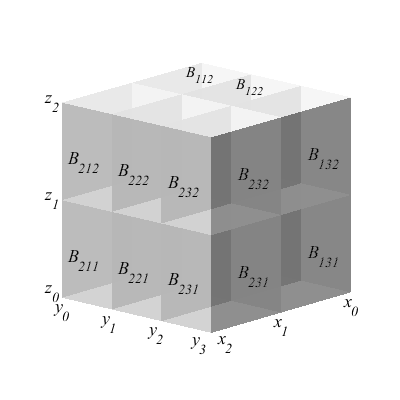
\includegraphics[trim=0cm 1.5cm 0cm 1.5cm, clip]{11_7_1_box_labeling.png}}
\end{center}
%\caption{A partitioned three-dimensional domain.}
%\label{F:11.7.Box_domain_2}
%\end{figure}
\end{activitySolution}
\aftera


%This process of partitioning that we carried out in Activity \ref{A:11.7.1} is the idea behind the triple Riemann sum.

\vspace*{5pt}
\nin \framebox{\hspace*{3 pt}
\parbox{6.25 in}{\textbf{The Triple Riemann Sum.} \begin{definition} Let $f = f(x,y,z)$ be a continuous function on a box $B = [a,b] \times [c,d] \times [r,s]$. The \textbf{triple Riemann sum of $f$ over $B$}\index{triple Riemann sum} is created as follows.
\begin{itemize}
\item Partition the interval $[a,b]$ into $m$ subintervals of equal length $\Delta x = \frac{b-a}{m}$. Let $x_0$, $x_1$, $\ldots$, $x_m$ be the endpoints of these subintervals, where $a = x_0<x_1<x_2 < \cdots < x_m = b$.
Do likewise with the interval $[c,d]$ using $n$ subintervals of equal length $\Delta y = \frac{d-c}{n}$ to generate $c = y_0<y_1<y_2 < \cdots < y_n = d$, and with the interval $[r,s]$ using $\ell$ subintervals of equal length $\Delta z = \frac{s-r}{\ell}$ to have $r = z_0<z_1<z_2 < \cdots < z_l = s$.
\item Let $B_{ijk}$ be the sub-box of $B$ with opposite vertices $(x_{i-1},y_{j-1},z_{k-1})$ and $(x_i, y_j, z_k)$ for $i$ between $1$ and $m$, $j$ between $1$ and $n$, and $k$ between 1 and $\ell$. The volume of each $B_{ijk}$ is $\Delta V = \Delta x \cdot \Delta y \cdot \Delta z$.
\item Let $(x_{ijk}^*, y_{ijk}^*, z_{ijk}^*)$ be a point in box $B_{ijk}$ for each $i$, $j$, and $k$. The resulting triple Riemann sum for $f$ on $B$ is
\[\sum_{i=1}^m \sum_{j=1}^n \sum_{k=1}^{\ell} f(x_{ijk}^*, y_{ijk}^*, z_{ijk}^*) \cdot \Delta V.\]
\end{itemize}
\end{definition}
} \hspace*{3 pt}}
\vspace*{5pt}

If $f(x,y,z)$ represents the mass density of the box $B$, then, as we saw in Preview Activity~\ref{PA:11.7}, the triple Riemann sum approximates the total mass of the box $B$. In order to find the exact mass of the box, we need to let the number of sub-boxes increase without bound (in other words, let $m$, $n$, and $\ell$ go to infinity); in this case, the finite sum of the mass approximations becomes the actual mass of the solid $B$.   More generally, we have the following definition of the triple integral.

\vspace*{5pt}
\nin \framebox{\hspace*{3 pt}
\parbox{6.25 in}{\textbf{The Triple Integral Over a Box.} \begin{definition} With following notation defined as in a triple Riemann sum, the \textbf{triple integral of $f$ over $B$}\index{triple integral} is
\[\iiint_B f(x,y,z) \, dV = \lim_{m,n,\ell \to \infty} \sum_{i=1}^m \sum_{j=1}^n \sum_{k=1}^{\ell} f(x_{ijk}^*, y_{ijk}^*, z_{ijk}^*) \cdot \Delta V. \]
\end{definition}
} \hspace*{3 pt}}
\vspace*{5pt}

As we noted earlier, if $f(x, y, z)$ represents the density of the solid $B$ at each point $(x, y, z)$, then
 \[M = \iiint_B f(x,y,z) \, dV\]
 is the mass of $B$.\index{mass!of a solid}  Even more importantly, for any continuous function $f$ over the solid $B$, we can use a triple integral to determine the average value of $f$ over $B$, $f_{\mbox{\tiny{AVG}(B)}}$.  We note this generalization of our work with functions of two variables along with several others in the following important boxed information.  Note that each of these quantities may actually be considered over a general domain $S$ in $\R^3$, not simply a box, $B$.
 % is given by 
%$$f_{\mbox{\tiny{AVG}(B)}} = \frac{1}{V(B)} \iiint_B f(x,y,z) \, dV,$$
%where $V(B)$ is the volume of the box $B$.

%Also, as with double integrals, if we want to integrate over a region that is not a box, we enclose the region in a rectangular box and assume the density is 0 everywhere inside the box that is outside the region. Similarly, we can use triple integrals to find the volume of a solid, the average value of a function, and the center of mass of a solid with variable density:

\vspace*{5pt}
\nin \framebox{\hspace*{3 pt}
\parbox{6.25 in}{\begin{itemize}
\item The triple integral
\[\displaystyle V(S) = \iiint_S 1 \, dV\]
represents the \textbf{volume} of the solid $S$\index{volume of a solid}.
\item The \textbf{average value} of the function $f = f(x,y,x)$ over a solid domain $S$\index{average value over a solid} is given by
\[f_{\mbox{\tiny{AVG}(S)}} = \displaystyle \left(\frac{1}{V(S)} \right) \iiint_S f(x,y,z) \, dV,\]
where $V(S)$ is the volume of the solid $S$.
\item The \textbf{center of mass}\index{center of mass!of a solid} of the solid $S$ with density $\delta = \delta(x,y,z)$ is $(\overline{x}, \overline{y}, \overline{z})$, where
\[ \overline{x} = \frac{\iiint_S x \ \delta(x,y,z) \, dV}{M}, \ \ \  \overline{y} = \frac{\iiint_S y \ \delta(x,y,z) \, dV}{M}, \ \ \  \overline{z} = \frac{\iiint_S z \ \delta(x,y,z) \, dV}{M},\]
and $M = \displaystyle \iiint_S \delta(x,y,z) \, dV$ is the mass of the solid $S$.
\end{itemize}
} \hspace*{3 pt}}
\vspace*{5pt}


In the Cartesian coordinate system, the volume element $dV$ is $dz \, dy \, dx$, and, as a consequence, a triple integral of a function $f$ over a box $B = [a,b] \times [c,d] \times [r,s]$ in Cartesian coordinates can be evaluated as an iterated integral of the form
\[\iiint_B f(x,y,z) \, dV = \int_a^b \int_c^d \int_r^s f(x,y,z) \, dz \, dy \, dx.\]

If we want to evaluate a triple integral as an iterated integral over a solid $S$ that is not a box, then we need to describe the solid in terms of variable limits.

%\begin{activity} \label{A:11.7.2} Evaluate the triple integral of $f(x,y,z) = x-y+2z$ over the box $B = [0,2] \times [1,4] \times [-2,3]$.


\end{activity}
\begin{smallhint}

\end{smallhint}
\begin{bighint}

\end{bighint}
\begin{activitySolution}
As an iterated integral we have
\begin{align*}
\int \int \int_B f(x,y,z) \, dV &= \int_{-2}^3 \int_1^4 \int_0^2 x-y+2z \, dz \, dy \, dx \\
	&= \int_{-2}^3 \int_1^4 \left. \left[ (x-y)z+z^2\right] \right|_0^2 \, dy \, dx \\
	&= \int_{-2}^3 \int_1^4 2(x-y)+4 \, dy \, dx \\
	&= \int_{-2}^3 \left. \left[2xy-y^2+4y\right] \right|_1^4 \, dx \\
	&= \int_{-2}^3 6x-3 \, dx \\
	&= \left. \left[3x^2-3x\right] \right|_{-2}^3 \\
	&= 0.
\end{align*}
\end{activitySolution}
\aftera


\begin{activity} \label{A:11.7.3} 

\ba
	\item Set up and evaluate the triple integral of $f(x,y,z) = x-y+2z$ over the box $B = [-2,3] \times [1,4] \times [0,2]$.

	\item Let $S$ be the solid cone bounded by $z = \sqrt{x^2+y^2}$ and $z=3$. A picture of $S$ is shown at right in Figure \ref{F:11.7.Cone_and_Cone_proj}. Our goal in what follows is to set up an iterated integral of the form
\begin{equation} \label{eq:11.7.TI_not_box}
\int_{x=?}^{x=?} \int_{y=?}^{y=?} \int_{z=?}^{z=?} \delta(x,y,z) \, dz \, dy \, dx
\end{equation}
to represent the mass of $S$ in the setting where $\delta(x,y,z)$ tells us the density of $S$ at the point $(x,y,z)$. Our particular task is to find the limits on each of the three integrals.
\begin{figure}[ht]
\begin{center}
%\resizebox{!}{2.4in}{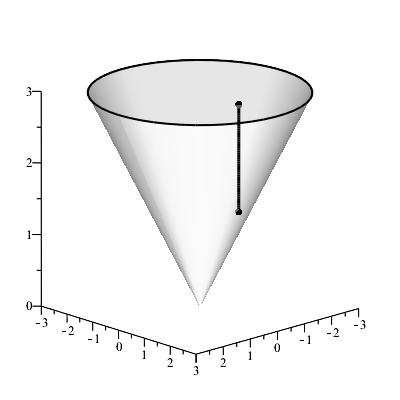
\includegraphics[trim=0cm 1cm 0cm 1.5cm, clip]{11_7_Cone_ex}}
    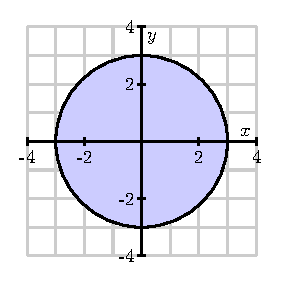
\includegraphics{figures/fig_11_7_cone_project.eps}
  \hspace{1.0in}
%\resizebox{!}{2.4in}{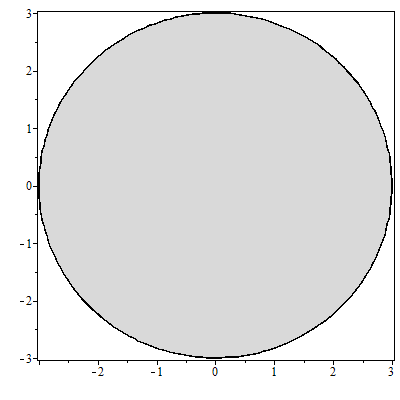
\includegraphics{11_7_Cone_proj}}
  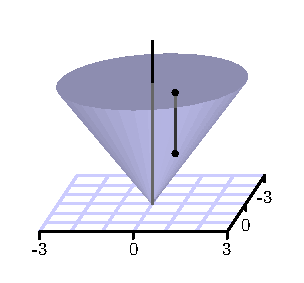
\includegraphics{figures/fig_11_7_cone.eps}
\caption{At right, the cone; at left, its projection.}
\label{F:11.7.Cone_and_Cone_proj}
\end{center}
\end{figure}
%crop graphics in animate trim=<left> <bottom> <right> <top>, clip with includegraphics

	\begin{enumerate}[i.]
	\item If we think about slicing up the solid, we can consider slicing the domain of the solid's projection onto the $xy$-plane (just as we would slice a two-dimensional region in $\R^2$), and then slice in the $z$-direction as well. The projection of the solid is onto the $xy$-plane is shown at left in Figure \ref{F:11.7.Cone_and_Cone_proj}. If we decide to first slice the domain of the solid's projection perpendicular to the $x$-axis, over what range of constant $x$-values would we have to slice?  

    \item If we continue with slicing the domain, what are the limits on $y$ on a typical slice?  How do these depend on $x$?   What, therefore, are the limits on the middle integral? 
    
    \item Finally, now that we have thought about slicing up the two-dimensional domain that is the projection of the cone, what are the limits on $z$ in the innermost integral? Note that over any point $(x,y)$ in the plane, a vertical slice in the $z$ direction will involve a range of values from the cone itself to its flat top.  In particular, observe that at least one of these limits is not constant but depends on $x$ and $y$.

    \item In conclusion, write an iterated integral of the form (\ref{eq:11.7.TI_not_box}) that represents the mass of the cone $S$.

	\end{enumerate}

    \ea

\end{activity}

\begin{smallhint}

\end{smallhint}
\begin{bighint}

\end{bighint}
\begin{activitySolution}
\ba
    
\item
As an iterated integral we have
\begin{align*}
\int \int \int_B f(x,y,z) \, dV &= \int_{-2}^3 \int_1^4 \int_0^2 x-y+2z \, dz \, dy \, dx \\
	&= \int_{-2}^3 \int_1^4 \left. \left[ (x-y)z+z^2\right] \right|_0^2 \, dy \, dx \\
	&= \int_{-2}^3 \int_1^4 2(x-y)+4 \, dy \, dx \\
	&= \int_{-2}^3 \left. \left[2xy-y^2+4y\right] \right|_1^4 \, dx \\
	&= \int_{-2}^3 6x-3 \, dx \\
	&= \left. \left[3x^2-3x\right] \right|_{-2}^3 \\
	&= 0.
\end{align*}

    
\item 
	\begin{enumerate}[i.]
	\item The values of $x$ run from $-3$ to $3$.

    \item The projection of the cone $S$ onto the $xy$-plane is image of the top of the cone, or the equation $\sqrt{x^2+y^2} = 3$. This is the circle $x^2+y^2 = 9$. The limits on $y$ are from the bottom of the circle to the top, or $-\sqrt{9-x^2} \leq y \leq \sqrt{9-x^2}$. 

	\item Notice that the smallest value of $z$ on each slice is on the cone, and the largest value of $z$ is on the plane $z=3$. So the limits on $z$ are $\sqrt{x^2+y^2} \leq z \leq 3$.
	
    \item An iterated integral that represents the mass of the cone $S$ is
\[  \int_{-3}^3 \int_{-\sqrt{9-x^2}}^{\sqrt{9-x^2}} \int_{\sqrt{x^2+y^2}}^{3} \delta(x,y,z) \, dz \, dy \, dx.\]
	\end{enumerate}
    \ea
\end{activitySolution}

\aftera



\noindent \textbf{Note well: } When setting up iterated integrals, the limits on a given variable can be {\em only} in terms of the remaining variables.  In addition, there are multiple different ways we can choose to set up such an integral.  For example, two possibilities for iterated integrals that represent a triple integral $\ds \iiint_S f(x,y,z) \, dV$ over a solid $S$ are
\begin{itemize}
\item $\ds \int_a^b \int_{g_1(x)}^{g_2(x)} \int_{h_1(x,y)}^{h_2(x,y)} f(x,y,z) \, dz \, dy \, dx$
%\item $\ds \int_c^d \int_{p_1(y)}^{p_2(y)} \int_{h_1(x,y)}^{h_2(x,y)} f(x,y,z) \, dz \, dx \, dy$
%\item $\ds \int_a^b \int_{g_1(x)}^{g_2(x)} \int_{h_1(x,z)}^{h_2(x,z)} f(x,y,z) \, dy \, dz \, dx$
\item $\ds \int_r^s \int_{p_1(z)}^{p_2(z)} \int_{q_1(x,z)}^{q_2(x,z)} f(x,y,z) \, dy \, dx \, dz$
%\item $\ds \int_c^d \int_{g_1(y)}^{g_2(y)} \int_{h_1(y,z)}^{h_2(y,z)} f(x,y,z) \, dx \, dz \, dy$
%\item $\ds \int_r^s \int_{g_1(z)}^{g_2(z)} \int_{h_1(y,z)}^{h_2(y,z)} f(x,y,z) \, dx \, dy \, dz$
\end{itemize}
where $g_1$, $g_2$, $h_1$, $h_2$, $p_1$, $p_2$, $q_1$, and $q_2$ are functions of the indicated variables.  There are four other options beyond the two stated here, since the variables $x$, $y$, and $z$ can (theoretically) be arranged in any order.   Of course, in many circumstances, an insightful choice of variable order will make it easier to set up an iterated integral, just as was the case when we worked with double integrals.

\begin{example} \label{ex:11.7.Tetrahedron_mass} Find the mass of the tetrahedron in the first octant bounded by the coordinate planes and the plane $x + 2 y + 3 z = 6$ if the density at point $(x,y,z)$ is given by $\delta(x, y, z) = x + y + z$. A picture of the solid tetrahedron is shown at left in Figure \ref{F:11.7.Tetrahedron_ex}.
\begin{figure}[ht]
\begin{center}
  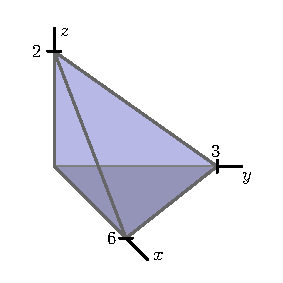
\includegraphics{figures/fig_11_7_tetrahedron.eps}
\hspace{1.0in}
%\resizebox{!}{2.2in}{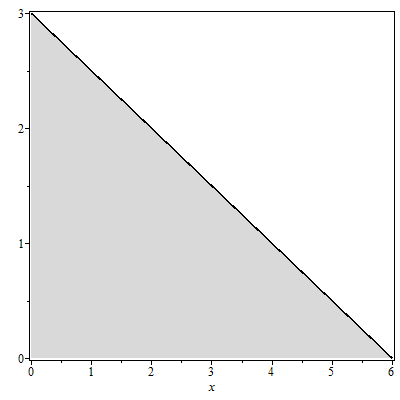
\includegraphics{11_7_Tetrahedron_proj}}
  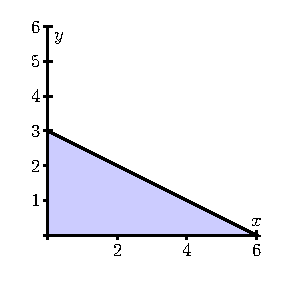
\includegraphics{figures/fig_11_7_tetrahedron_project.eps}
\caption{The tetrahedron and its projection.}
\label{F:11.7.Tetrahedron_ex}
\end{center}
\end{figure}
%crop graphics in animate trim=<left> <bottom> <right> <top>, clip with includegraphics

We find the mass, $M$, of the tetrahedron by the triple integral
\[ M = \iiint_S \delta(x,y,z) \, dV,\]
where $S$ is the solid tetrahedron described above. In this example, we choose to integrate with respect to $z$ first for the innermost integral. The top of the tetrahedron is given by the equation
\[x + 2 y + 3 z = 6;\]
 solving for $z$ then yields
\[z = \frac{1}{3}(6 - x - 2y).\]
The bottom of the tetrahedron is the $xy$-plane, so the limits on $z$ in the iterated integral will be $0 \leq z \leq \frac{1}{3}(6-x-2y)$.

To find the bounds on $x$ and $y$ we project the tetrahedron onto the $xy$-plane; this corresponds to setting $z = 0$ in the equation $z = \frac{1}{3}(6 - x - 2y)$. The resulting relation between $x$ and $y$ is
\[x + 2 y = 6.\]
The right image in Figure \ref{F:11.7.Tetrahedron_ex} shows the projection of the tetrahedron onto the $xy$-plane.

If we choose to integrate with respect to $y$ for the middle integral in the iterated integral, then the lower limit on $y$ is the $x$-axis and the upper limit is the hypotenuse of the triangle. Note that the hypotenuse joins the points $(6,0)$ and $(0,3)$ and so has equation $y = 3 - \frac{1}{2}x$. Thus, the bounds on $y$ are $0 \leq y \leq 3 - \frac{1}{2}x$. Finally, the $x$ values run from 0 to 6, so the iterated integral that gives the mass of the tetrahedron is
\begin{equation}
M = \int_{0}^{6} \int_{0}^{3-(1/2)x} \int_{0}^{(1/3)(6-x-2y)} x+y+z \, dz \, dy \, dx. \label{eq:11.7.Tetrahedron_mass}
\end{equation}
Evaluating the triple integral gives us
\begin{align*}
M & = \int_{0}^{6} \int_{0}^{3-(1/2)x} \int_{0}^{(1/3)(6-x-2y)} x+y+x \, dz \, dy \, dx  \\
    &= \int_{0}^{6} \int_{0}^{3-(1/2)x} \left[xz+yz+\frac{z}{2}\right]\biggm|_{0}^{(1/3)(6-x-2y)} \, dy \, dx \\
	&= \int_{0}^{6} \int_{0}^{3-(1/2)x} \frac{4}{3}x - \frac{5}{18}x^2 - \frac{}{9}xy + \frac{2}{3}y - \frac{4}{9}y^2 + 2 \, dy \, dx \\
	&= \int_{0}^{6} \left[\frac{4}{3}xy - \frac{5}{18}x^2y - \frac{7}{18}xy^2 + \frac{1}{3}y^2 - \frac{4}{27}y^3 + 2y \right]\biggm|_{0}^{3-(1/2)x}  \, dx \\
	&= \int_{0}^{6} 5 + \frac{1}{2}x - \frac{7}{12}x^2 + \frac{13}{216}x^3 \, dx \\
	&=  \left[5x + \frac{1}{4}x^2 - \frac{7}{36}x^3 + \frac{13}{864}x^4 \right] \biggm|_{0}^{6} \\
	&= \frac{33}{2}.
\end{align*}
\end{example}

Setting up limits on iterated integrals can require considerable geometric intuition.  It is important to not only create carefully labeled figures, but also to think about how we wish to slice the solid.  Further, note that when we say ``we will integrate first with respect to $x$,'' by ``first'' we are referring to the innermost integral in the iterated integral.  The next activity explores several different ways we might set up the integral in the preceding example.

\begin{activity} \label{A:11.7.4} There are several other ways we could have set up the integral to give the mass of the tetrahedron in Example \ref{ex:11.7.Tetrahedron_mass}.
	\ba
	\item How many different iterated integrals could be set up that are equal to the integral in Equation~(\ref{eq:11.7.Tetrahedron_mass})?



	\item Set up an iterated integral, integrating first with respect to $z$, then $x$, then $y$ that is equivalent to the integral in Equation~(\ref{eq:11.7.Tetrahedron_mass}).  Before you write down the integral, think about Figure~\ref{F:11.7.Tetrahedron_ex}, and draw an appropriate two-dimensional image of an important projection.

	\item Set up an iterated integral, integrating first with respect to $y$, then $z$, then $x$ that is equivalent to the integral in Equation~(\ref{eq:11.7.Tetrahedron_mass}).  As in (b), think carefully about the geometry first.

	\item Set up an iterated integral, integrating first with respect to $x$, then $y$, then $z$ that is equivalent to the integral in Equation~(\ref{eq:11.7.Tetrahedron_mass}).



	\ea

\end{activity}
\begin{smallhint}

\end{smallhint}
\begin{bighint}

\end{bighint}
\begin{activitySolution}
	\ba
	\item We can choose any of $x$, $y$, or $z$ to be our innermost variable of integration. Once we make that choice, there are two variables left for the middle integral, and then only one for the outermost integral. So we have $3 \times 2 \times 1 = 6$ different iterated integrals that are equal to the integral in (\ref{eq:11.7.Tetrahedron_mass}).

	\item If we integrate with respect to $z$ first, the limits on $z$ will remain the same as in (\ref{eq:11.7.Tetrahedron_mass}). The projection of the tetrahedron onto the $xy$-plane is still bounded by the line $x+2y=6$, and this region can be described by the inequalities $0 \leq x \leq 6-2y$ and $0 \leq y \leq 3$. So our iterated integral is  
\[\int_{0}^{3} \int_{0}^{6-2y} \int_{0}^{(1/3)(6-x-2y)} x+y+z \, dz \, dx \, dy.\]
		
	\item If we integrate with respect to $y$ first, the lower limit on $y$ is 0 and the upper limit is the face of the tetrahedron, $y = \frac{1}{2}(6-3z-x)$. The projection of the tetrahedron onto the $xz$-plane is bounded by the coordinate axes and the line $x+3z=6$. This region can be described by the inequalities $0 \leq z \leq \frac{1}{3}(6-x)$ and $0 \leq x \leq 6$. So our iterated integral is 
\[\int_{0}^{6} \int_{0}^{1/3(6-x)} \int_{0}^{\frac{1}{2}(6-3z-x)} x+y+z \, dy \, dz \, dx.\]


	\item If we integrate with respect to $x$ first, the lower limit on $x$ is 0 and the upper limit is the face of the tetrahedron, $x = 6-3z-2y$. The projection of the tetrahedron onto the $yz$-plane is bounded by the coordinate axes and the line $2y+3z=6$. This region can be described by the inequalities $0 \leq y \leq \frac{1}{2}(6-3z)$ and $0 \leq z \leq 2$. So our iterated integral is 
\[\int_{0}^{2} \int_{0}^{1/2(6-3z)} \int_{0}^{6-3z-2y} x+y+z \, dx \, dy \, dz.\]

	\ea
\end{activitySolution}
\aftera


%\begin{activity} \label{A:11.7.5} Consider the solid $S$ that is bounded by the parabolic cylinder $y = x^2$ and the planes $z=0$ and $z=1-y$ as shown in Figure \ref{F:11.7.TI_Example_2}. 
\begin{figure}[ht]
\begin{center}
%\resizebox{!}{2.0in}{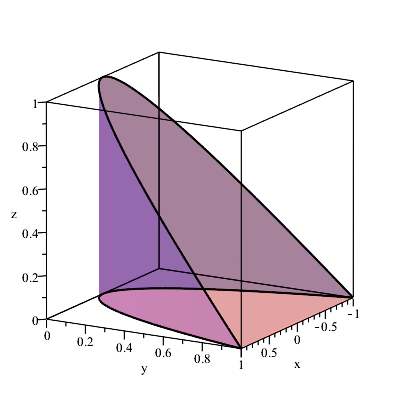
\includegraphics{11_7_TI_Example_2}}
  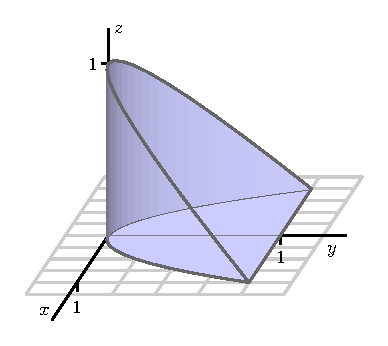
\includegraphics{figures/fig_11_7_solid.eps}
\end{center}
\caption{The solid bounded by $y = x^2$ and the planes $z=0$ and $z=1-y$.}
\label{F:11.7.TI_Example_2}
\end{figure}

Assume the density of $S$ is given by $\delta(x,y,z) = z$
    \ba
    \item Set up (but do not evaluate) an iterated integral that represents the mass of $S$.  Integrate first with respect to $z$, then $y$, then $x$  A picture of the projection of $S$ onto the $xy$-plane is shown in Figure \ref{F:11.7.TI_Example_2_xy}.

    \item Set up (but do not evaluate) an iterated integral that represents the mass of $S$.  In this case, integrate first with respect to $y$, then $z$, then $x$.  A picture of the projection of $S$ onto the $xz$-plane is shown in Figure \ref{F:11.7.TI_Example_2_xz}.


	\item Set up (but do not evaluate) an iterated integral that represents the mass of $S$.  A picture of the projection of $S$ onto the $yz$-plane is shown in Figure \ref{F:11.7.TI_Example_2_yz}.

	\item Which of these three orders of integration is the most natural to you?  Why?

	\ea

\begin{figure}[ht]
\begin{center}
\begin{minipage}{1.75in}
\begin{center}
%\resizebox{!}{1.7in}{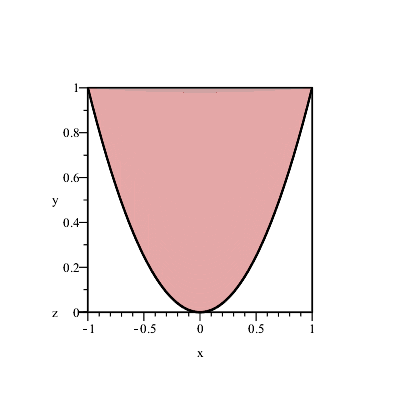
\includegraphics{11_7_TI_Example_2_xy}}
  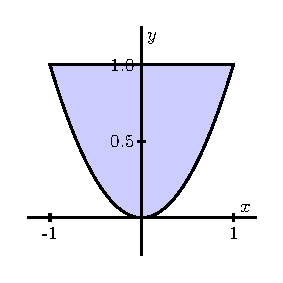
\includegraphics{figures/fig_11_7_solid_proj_1.eps}
\end{center}
\caption{Projecting $S$ onto the $xy$-plane.}
\label{F:11.7.TI_Example_2_xy}
\end{minipage} \hspace{0.1in}
\begin{minipage}{1.75in}
\begin{center}
%\resizebox{!}{1.7in}{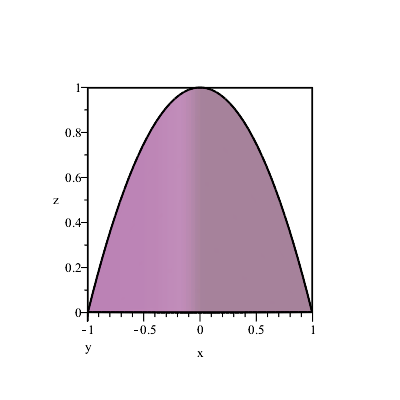
\includegraphics{11_7_TI_Example_2_xz}}
  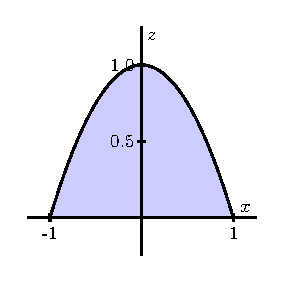
\includegraphics{figures/fig_11_7_solid_proj_2.eps}
\end{center}
\caption{Projecting $S$ onto the $xz$-plane.}
\label{F:11.7.TI_Example_2_xz}
\end{minipage} \hspace{0.1in}
\begin{minipage}{1.75in}
\begin{center}
%\resizebox{!}{1.7in}{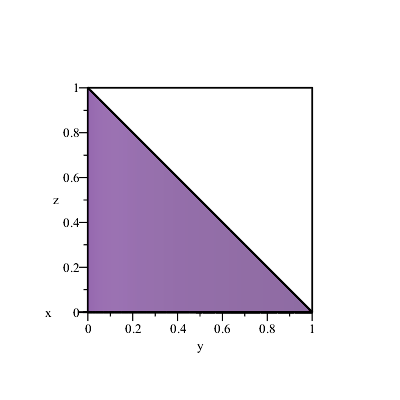
\includegraphics{11_7_TI_Example_2_yz}}
  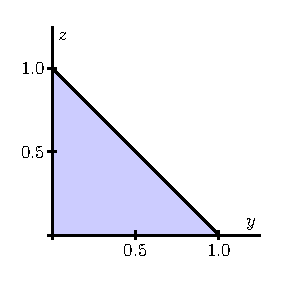
\includegraphics{figures/fig_11_7_solid_proj_3.eps}
\end{center}
\caption{Projecting $S$ onto the $yz$-plane.}
\label{F:11.7.TI_Example_2_yz}
\end{minipage}
\end{center}
\end{figure}


\end{activity}
\begin{smallhint}

\end{smallhint}
\begin{bighint}

\end{bighint}
\begin{activitySolution}
    \ba
    \item The iterated integral is 
\[\int_{-1}^{1} \int_{x^2}^{1} \int_{0}^{1-y} z \, dz \, dy \, dx.\]

    \item The iterated integral is 
\[\int_{0}^{1} \int_{0}^{1-x^2} \int_{x^2}^{1} z \, dy \, dz \, dx.\]

	\item The iterated integral is 
\[\int_{0}^{1} \int_{0}^{z} \int_{-\sqrt{y}}^{\sqrt{y}} z \, dx \, dy \, dz.\]

	\ea
\end{activitySolution}
\aftera


Now that we have begun to understand how to set up iterated triple integrals, we can apply them to determine important quantities, such as those found in the next activity.

\begin{activity} \label{A:11.7.6} A solid $S$ is bounded below by the square $z=0$, $-1 \leq x \leq 1$, $-1 \leq y \leq 1$ and above by the surface $z = 2-x^2-y^2$. A picture of the solid is shown in Figure \ref{F:11.7.COM3D}.
\begin{figure}[ht]
\begin{center}
%\resizebox{!}{2.0in}{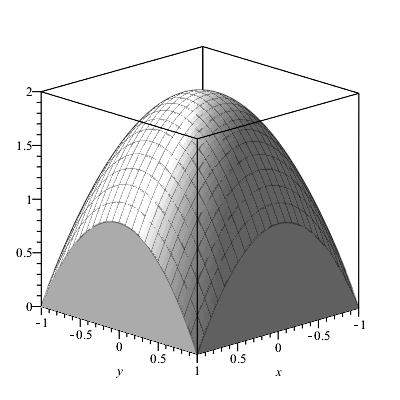
\includegraphics[trim=0cm 0.5cm 0cm 1cm, clip]{11_7_COM3D}}
  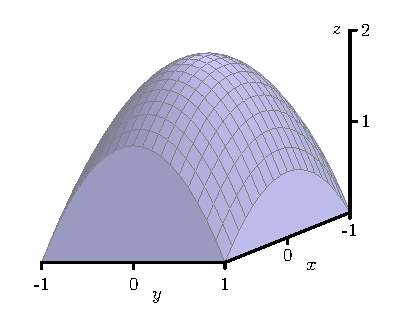
\includegraphics{figures/fig_11_7_volume.eps}
\end{center}
\caption{The solid bounded by the surface $z = 2-x^2-y^2$.}
\label{F:11.7.COM3D}
\end{figure}
%crop graphics in animate trim=<left> <bottom> <right> <top>, clip with includegraphics

    \ba
    \item Set up (but do not evaluate) an iterated integral to find the volume of the solid $S$.

    \item Set up (but do not evaluate) iterated integral expressions that will tell us the center of mass of $S$, if the density at point $(x,y,z)$ is $\delta(x,y,z)=x^2+1$.

    \item Set up (but do not evaluate) an iterated integral to find the average density on $S$ using the density function from part (b).

    \item Use technology appropriately to evaluate the iterated integrals you determined in (a), (b), and (c); does the location you determined for the center of mass make sense?

    \ea

\end{activity}
\begin{smallhint}

\end{smallhint}
\begin{bighint}

\end{bighint}
\begin{activitySolution}
    \ba
    \item We integrate first with respect to $z$, so that $0 \leq z \leq 2-x^2-y^2$. The projection of the surface onto the $xy$-plane is the square, so an iterated integral that gives the volume of $S$ is 
\[\int_{-1}^1 \int_{-1}^1 \int_0^{2-x^2-y^2} dz \, dy \, dx.\]

    \item The center of mass of $S$ is $(\overline{x}, \overline{y}, \overline{z})$, where 
\begin{align*}
\overline{x} &= \frac{\int_{-1}^1 \int_{-1}^1 \int_0^{2-x^2-y^2} x(x^2+1) \, dz \, dy \, dx}{\int_{-1}^1 \int_{-1}^1 \int_0^{2-x^2-y^2} x^2+1 \, dz \, dy \, dx} \\
\overline{y} &= \frac{\int_{-1}^1 \int_{-1}^1 \int_0^{2-x^2-y^2} y(x^2+1) \, dz \, dy \, dx}{\int_{-1}^1 \int_{-1}^1 \int_0^{2-x^2-y^2} x^2+1 \, dz \, dy \, dx} \\
\overline{z} &= \frac{\int_{-1}^1 \int_{-1}^1 \int_0^{2-x^2-y^2} z(x^2+1) \, dz \, dy \, dx}{\int_{-1}^1 \int_{-1}^1 \int_0^{2-x^2-y^2} x^2+1 \, dz \, dy \, dx}.
\end{align*}

    \item The average density is given by 
\[\frac{\int_{-1}^1 \int_{-1}^1 \int_0^{2-x^2-y^2} x^2+1 \, dz \, dy \, dx}{\int_{-1}^1 \int_{-1}^1 \int_0^{2-x^2-y^2} 1 \, dz \, dy \, dx}.\]

	\item The volume of the solid is $\frac{16}{3}$, the center of mass is $\left(0,0,\frac{94}{133}\right)$, and the average density is $\frac{19}{15}$. Given the symmetry, we should expect $\overline{x}$ and $\overline{y}$ to be 0. Since the bulk of the mass is nearer to the $xy$-plane, it makes sense that $\overline{z}$ is less than 1.  
    \ea
\end{activitySolution}
\aftera


%\begin{activity} \label{A:11.7.7} Set up an iterated integral or integrals that will find the average sum of the numbers $x$, $y$, and $z$ if $y$ is between 0 and 2, $x$ is greater than or equal to 0 but cannot exceed $2y$, and $z$ is greater than or equal to 0 but cannot exceed $x+y$.

\end{activity}
\begin{smallhint}

\end{smallhint}
\begin{bighint}

\end{bighint}
\begin{activitySolution}
We want the average value of the sum $x+y+z$ over the region described. This average value is given by 
\[\frac{\int_0^2 \int_0^{2y} \int_0^{x+y} x+y+z \, dz \, dx \, dy}{\int_0^2 \int_0^{2y} \int_0^{x+y} 1 \, dz \, dx \, dy}.\]
\end{activitySolution}
\aftera




\begin{summary}
\item Let $f = f(x,y,z)$ be a continuous function on a box $B = [a,b] \times [c,d] \times [r,s]$. 
%The triple Riemann sum of $f$ over $B$ is created as follows.
%\begin{itemize}
%\item Partition the interval $[a,b]$ into $m$ subintervals of equal length $\Delta x = \frac{b-a}{m}$. Let $x_0$, $x_1$, $\ldots$, $x_m$ be the endpoints of these subintervals, where $a = x_0<x_1<x_2 < \cdots < x_m = b$.
%\item Partition the interval $[c,d]$ into $n$ subintervals of equal length $\Delta y = \frac{d-c}{n}$. Let $y_0$, $y_1$, $\ldots$, $y_n$ be the endpoints of these subintervals, where $c = y_0<y_1<y_2 < \cdots < y_n = d$.
%\item Partition the interval $[r,s]$ into $l$ subintervals of equal length $\Delta z = \frac{s-r}{l}$. Let $z_0$, $z_1$, $\ldots$, $z_l$ be the endpoints of these subintervals, where $r = z_0<z_1<z_2 < \cdots < z_l = s$.
%\item Let $B_{ijk}$ be the sub-box of $B$ with opposite vertices $(x_{i-1},y_{j-1},z_{l-1})$ and $(x_i, y_j, z_k)$ for $i$ between $1$ and $m$, $j$ between $1$ and $n$, and $k$ between 1 and $l$. The volume of $B_{ijk}$ is $\Delta V = \Delta x \cdot \Delta y \cdot \Delta z$.
%\item Let $(x_{ijk}^*, y_{ijk}^*, z_{ijk}^*)$ be a point in box $B_{ijk}$ for each $i$, $j$, and $k$. Then a triple Riemann sum for $f$ on $B$ is
%\[\sum_{i=1}^m \sum_{j=1}^n \sum_{k=1}^l f(x_{ijk}^*, y_{ijk}^*, z_{ijk}^*) \cdot \Delta V.\]
%\end{itemize}
 The triple integral of $f$ over $B$ is defined as
\[\iiint_B f(x,y,z) \, dV = \lim_{\Delta V \to 0} \sum_{i=1}^m \sum_{j=1}^n \sum_{k=1}^l f(x_{ijk}^*, y_{ijk}^*, z_{ijk}^*) \cdot \Delta V,\]
where the triple Riemann sum is defined in the usual way. %If $f$ is defined over some solid $S$, we enclose $S$ in a box $B$ and define $f$ to have the value 0 outside of $B$. In this case,
%\[\iiint_S f(x,y,z) \, dV = \iiint_B f(x,y,z) \, dV.\]
The definition of the triple integral naturally extends to non-rectangular solid regions $S$.
\item The triple integral $\ds \iiint_S f(x,y,z) \, dV$ can tell us
    \begin{itemize}
    \item[-] the volume of the solid $S$ if $f(x,y,z) = 1$,
    \item[-] the mass of the solid $S$ if $f$ represents the density of $S$ at the point $(x,y,z)$.
    \end{itemize}
Moreover,     \[f_{\mbox{\tiny{AVG}(S)}} = \displaystyle \frac{1}{V(S)} \iiint_S f(x,y,z) \, dV,\] is the average value of $f$ over $S$.
\end{summary}

\nin \hrulefill

\begin{exercises} 

\item Consider the solid $S$ that is bounded by the parabolic cylinder $y = x^2$ and the planes $z=0$ and $z=1-y$ as shown in Figure \ref{F:11.7.TI_Example_2}. 
\begin{figure}[ht]
\begin{center}
%\resizebox{!}{2.0in}{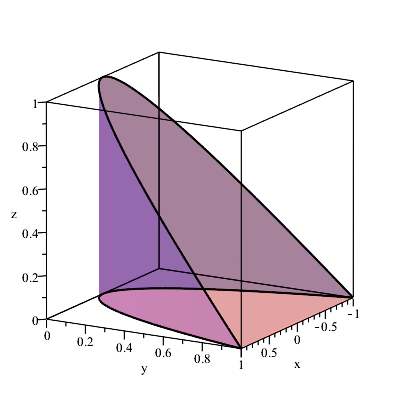
\includegraphics{11_7_TI_Example_2}}
  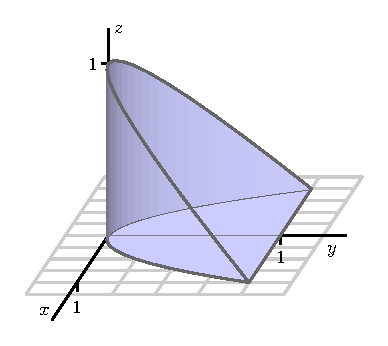
\includegraphics{figures/fig_11_7_solid.eps}
\end{center}
\caption{The solid bounded by $y = x^2$ and the planes $z=0$ and $z=1-y$.}
\label{F:11.7.TI_Example_2}
\end{figure}

Assume the density of $S$ is given by $\delta(x,y,z) = z$
    \ba
    \item Set up (but do not evaluate) an iterated integral that represents the mass of $S$.  Integrate first with respect to $z$, then $y$, then $x$.  A picture of the projection of $S$ onto the $xy$-plane is shown in Figure \ref{F:11.7.TI_Example_2_xy}.

    \item Set up (but do not evaluate) an iterated integral that represents the mass of $S$.  In this case, integrate first with respect to $y$, then $z$, then $x$.  A picture of the projection of $S$ onto the $xz$-plane is shown in Figure \ref{F:11.7.TI_Example_2_xz}.

	\item Set up (but do not evaluate) an iterated integral that represents the mass of $S$.  For this integral, integrate first with respect to $x$, then $y$, then $z$.  A picture of the projection of $S$ onto the $yz$-plane is shown in Figure \ref{F:11.7.TI_Example_2_xz}.

	\item Which of these three orders of integration is the most natural to you?  Why?

	\ea

\begin{figure}[ht]
\begin{center}
\begin{minipage}{1.75in}
\begin{center}
%\resizebox{!}{1.7in}{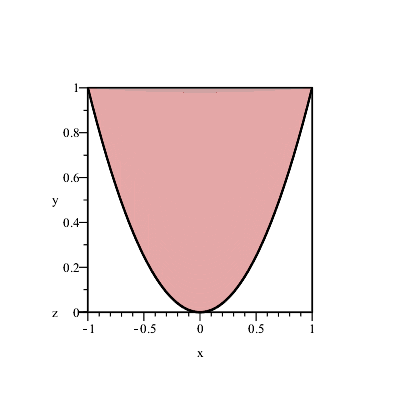
\includegraphics{11_7_TI_Example_2_xy}}
  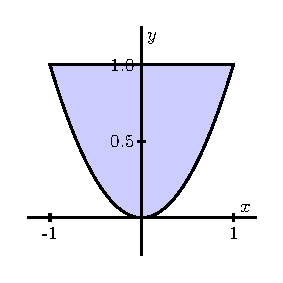
\includegraphics{figures/fig_11_7_solid_proj_1.eps}
\end{center}
\caption{Projecting $S$ onto the $xy$-plane.}
\label{F:11.7.TI_Example_2_xy}
\end{minipage} \hspace{0.1in}
\begin{minipage}{1.75in}
\begin{center}
%\resizebox{!}{1.7in}{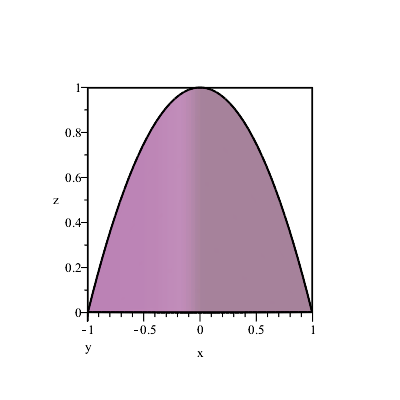
\includegraphics{11_7_TI_Example_2_xz}}
  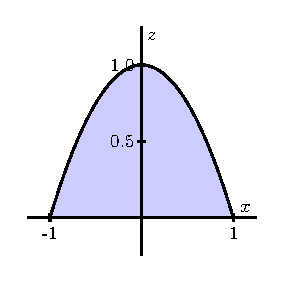
\includegraphics{figures/fig_11_7_solid_proj_2.eps}
\end{center}
\caption{Projecting $S$ onto the $xz$-plane.}
\label{F:11.7.TI_Example_2_xz}
\end{minipage} \hspace{0.1in}
\begin{minipage}{1.75in}
\begin{center}
%\resizebox{!}{1.7in}{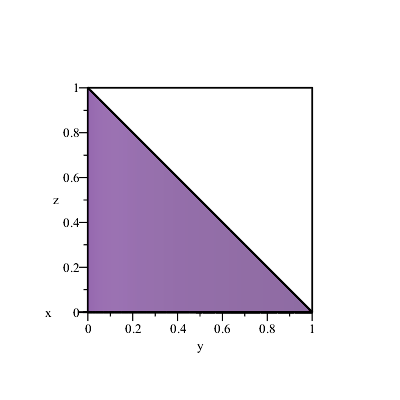
\includegraphics{11_7_TI_Example_2_yz}}
  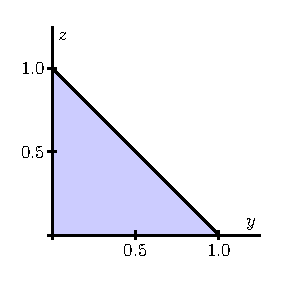
\includegraphics{figures/fig_11_7_solid_proj_3.eps}
\end{center}
\caption{Projecting $S$ onto the $yz$-plane.}
\label{F:11.7.TI_Example_2_yz}
\end{minipage}
\end{center}
\end{figure}

\begin{exerciseSolution}
    \ba
    \item The iterated integral is 
\[\int_{-1}^{1} \int_{x^2}^{1} \int_{0}^{1-y} z \, dz \, dy \, dx.\]

    \item The iterated integral is 
\[\int_{-1}^{1} \int_{0}^{1-x^2} \int_{x^2}^{1-z} z \, dy \, dz \, dx.\]

	\item The iterated integral is 
\[\int_{0}^{1} \int_{0}^{1-z} \int_{-\sqrt{y}}^{\sqrt{y}} z \, dx \, dy \, dz.\]

	\ea
\end{exerciseSolution}

\item This problem asks you to investigate the average value of some different quantities.

	\ba
		\item Set up, but do not evaluate, an iterated integral expression whose value is the average sum of all real numbers $x$, $y$, and $z$ that have the following property: $y$ is between 0 and 2, $x$ is greater than or equal to 0 but cannot exceed $2y$, and $z$ is greater than or equal to 0 but cannot exceed $x+y$.
		\item Set up, but do not evaluate, an integral expression whose value represents the average value of the function $f(x,y,z) = x + y + z$ over the solid region in the first octant bounded by the surface $z = 4 - x - y^2$ and the coordinate planes $x=0$, $y=0$, $z=0$. 
		\item How are the quantities in (a) and (b) similar?  How are they different?
	\ea
	
\begin{exerciseSolution}
\ba
\item We want the average value of the sum $x+y+z$ over the region described. This average value is given by 
\[\frac{\int_0^2 \int_0^{2y} \int_0^{x+y} x+y+z \, dz \, dx \, dy}{\int_0^2 \int_0^{2y} \int_0^{x+y} 1 \, dz \, dx \, dy}.\]
\item We will integrate $x+y+z$ for $z$ from $0$ to $4-x-y^2$. To find the limits on $x$ and $y$, we project $z$ into the $x$-$y$ plane to the parabola $0 = 4 - x- y^2$ or $x = 4-y^2$. Since we are restricted to the first octant, the average value of $f(x,y,z)$ over this region is 
\[\frac{\int_0^2 \int_0^{4-y^2} \int_0^{4-x-y^2} x+y+z \, dz \, dx \, dy}{\int_0^2 \int_0^{4-y^2} \int_0^{4-x-y^2} 1 \, dz \, dx \, dy}.\]
\ea
\end{exerciseSolution}

\item Consider the solid that lies between the paraboloids $z = g(x,y) = x^2 + y^2$ and $z = f(x,y) = 8 - 3x^2 - 3y^2$.

	\ba
		\item By eliminating the variable $z$, determine the curve of intersection between the two paraboloids, and sketch this curve in the $x$-$y$ plane.
		\item Set up, but do not evaluate, an iterated integral expression whose value determine the mass of the solid, integrating first with respect to $x$, then $y$, then $z$. Assume the the solid's density is given by $\delta(x,y,z) = \frac{1}{x^2 + y^2 + z^2 + 1}$.
		\item Set up, but do not evaluate, iterated integral expressions whose values determine the mass of the solid using all possible remaining orders of integration. Use $\delta(x,y,z) = \frac{1}{x^2 + y^2 + z^2 + 1}$ as the density of the solid.
		\item Set up, but do not evaluate, iterated integral expressions whose values determine the center of mass of the solid. Again, assume the the solid's density is given by $\delta(x,y,z) = \frac{1}{x^2 + y^2 + z^2 + 1}$.
		\item Which coordinates of the center of mass can you determine \emph{without} evaluating any integral expression?  Why?
	\ea

\begin{exerciseSolution}
	\ba
		\item Setting $g(x,y)$ equal to $f(x,y)$ we see that the curve of intersection between the two paraboloids is given by $x^2+y^2 = 8-3x^2-3y^2$ or $x^2+y^2=2$. This is the circle centered at the origin with radius $\sqrt{2}$. 
		\item To find mass, we integrate density. An iterated integral whose value represent the mass of the solid is
\[\int_{-\sqrt{2}}^{\sqrt{2}} \int_{-\sqrt{2-x^2}}^{\sqrt{2-x^2}} \int_{x^2+y^2}^{8-3x^2-3y^2} \frac{1}{x^2 + y^2 + z^2 + 1} \, dz \, dy \, dx.\]
		\item If we interchange the orders of $y$ and $x$, then symmetry shows that the mass of the solid is given by 
\[\int_{-\sqrt{2}}^{\sqrt{2}} \int_{-\sqrt{2-y^2}}^{\sqrt{2-y^2}} \int_{x^2+y^2}^{8-3x^2-3y^2} \frac{1}{x^2 + y^2 + z^2 + 1} \, dz \, dx \, dy.\]
To integrate with respect to $y$ first, notice that the limits on $y$ will vary depending on the height. If $0 \leq z \leq 2$, then the limits on $y$ are determined by the paraboloid $z = x^2+y^2$. In this case we have $-\sqrt{z-x^2} \leq y \leq \sqrt{z-x^2}$. When we project this part of the surface onto the $x$-$z$ plane, the result is the parabola $z=x^2$. We want the region above this parabola and below $z=2$. If $2 \leq z \leq 8$, then the limits on $y$ are determined by the paraboloid $z = 8-3x^2-3y^2$. In this case we have $-\sqrt{8-z-3x^2} \leq y \leq \sqrt{8-z-3x^2}$. When we project this part of the surface onto the $x$-$z$ plane, the result is the parabola $z=8-3x^2$. We want the region below this parabola and above $z=2$. So the mass of the solid is given by 
\[\int_{-\sqrt{2}}^{\sqrt{2}} \int_{x^2}^{2} \int_{-\sqrt{z-x^2}}^{\sqrt{z-x^2}} \frac{1}{x^2 + y^2 + z^2 + 1} \, dy \, dz \, dx + \int_{-\sqrt{2}}^{\sqrt{2}} \int_{2}^{8-3x^2} \int_{-\sqrt{\frac{1}{3}(8-z-3x^2)}}^{\sqrt{\frac{1}{3}(8-z-3x^2)}} \frac{1}{x^2 + y^2 + z^2 + 1} \, dy \, dz \, dx .\]


Interchanging the orders of $x$ and $z$ shows that the mass of the solid is given by 
\[\int_{0}^{2} \int_{-\sqrt{z}}^{\sqrt{z}} \int_{-\sqrt{z-x^2}}^{\sqrt{z-x^2}} \frac{1}{x^2 + y^2 + z^2 + 1} \, dy \, dx \, dz + \int_{2}^{8} \int_{-\sqrt{\frac{1}{3}(8-z)}}^{\sqrt{\frac{1}{3}(8-z)}} \int_{-\sqrt{\frac{1}{3}(8-z-3x^2)}}^{\sqrt{\frac{1}{3}(8-z-3x^2)}} \frac{1}{x^2 + y^2 + z^2 + 1} \, dy \, dx \, dz .\]

Finally, we integrate with respect to $x$ first. The symmetry in the surface indicates that these integrals will be similar to ones with $y$ first. So the mass of the solid is also given by 
\[\int_{-\sqrt{2}}^{\sqrt{2}} \int_{y^2}^{2} \int_{-\sqrt{z-y^2}}^{\sqrt{z-y^2}} \frac{1}{x^2 + y^2 + z^2 + 1} \, dx \, dz \, dy + \int_{-\sqrt{2}}^{\sqrt{2}} \int_{2}^{8-3y^2} \int_{-\sqrt{\frac{1}{3}(8-z-3y^2)}}^{\sqrt{\frac{1}{3}(8-z-3y^2)}} \frac{1}{x^2 + y^2 + z^2 + 1} \, dx \, dz \, dy\]
and
\[\int_{0}^{2} \int_{-\sqrt{z}}^{\sqrt{z}} \int_{-\sqrt{z-y^2}}^{\sqrt{z-y^2}} \frac{1}{x^2 + y^2 + z^2 + 1} \, dx \, dy \, dz + \int_{2}^{8} \int_{-\sqrt{\frac{1}{3}(8-z)}}^{\sqrt{\frac{1}{3}(8-z)}} \int_{-\sqrt{\frac{1}{3}(8-z-3y^2)}}^{\sqrt{\frac{1}{3}(8-z-3y^2)}} \frac{1}{x^2 + y^2 + z^2 + 1} \, dx \, dy \, dz .\]

		\item If $M$ is the mass of the solid from part (b), then the center of mass $(\overline{x}, \overline{y}, \overline{z})$ is given by
\begin{align*}
\overline{x} &= \frac{1}{M} \int_{-\sqrt{2}}^{\sqrt{2}} \int_{-\sqrt{2-x^2}}^{\sqrt{2-x^2}} \int_{x^2+y^2}^{8-3x^2-3y^2} \frac{x}{x^2 + y^2 + z^2 + 1} \, dz \, dy \, dx  \\
\overline{y} &= \frac{1}{M} \int_{-\sqrt{2}}^{\sqrt{2}} \int_{-\sqrt{2-x^2}}^{\sqrt{2-x^2}} \int_{x^2+y^2}^{8-3x^2-3y^2} \frac{y}{x^2 + y^2 + z^2 + 1} \, dz \, dy \, dx \\
\overline{z} &= \frac{1}{M} \int_{-\sqrt{2}}^{\sqrt{2}} \int_{-\sqrt{2-x^2}}^{\sqrt{2-x^2}} \int_{x^2+y^2}^{8-3x^2-3y^2} \frac{z}{x^2 + y^2 + z^2 + 1} \, dz \, dy \, dx.
\end{align*}

		\item There is symmetry around the $z$-axis, so we should expect $\overline{z} = 0$. 
	\ea
\end{exerciseSolution}

\item In each of the following problems, your task is to 
	\begin{itemize}
	\item[(i)] sketch, by hand, the region over which you integrate
	\item[(ii)] set up iterated integral expressions which, when evaluated, will determine the value sought  
	\item[(iii)] use appropriate technology to evaluate each iterated integral expression you develop
	\end{itemize}
Note well:  in some problems you may be able to use a double rather than a triple integral, and polar coordinates may be helpful in some cases.	
\ba

	\item Consider the solid created by the region enclosed by the circular paraboloid $z = 4 - x^2 - y^2$ over the region $R$ in the $x$-$y$ plane enclosed by $y = -x$ and the circle $x^2 + y^2 = 4$ in the first, second, and fourth quadrants. 
	
	Determine the solid's volume.

    \item Consider the solid region that lies beneath the circular paraboloid $z = 9 - x^2 - y^2$ over the triangular region between $y = x$, $y = 2x$, and $y = 1$.   Assuming that the solid has its density at point $(x,y,z)$ given by $\delta(x,y,z) = xyz + 1$, measured in grams per cubic cm, determine the center of mass of the solid.

	\item In a certain room in a house, the walls can be thought of as being formed by the lines $y = 0$, $y = 12 + x/4$, $x = 0$, and $x = 12$, where length is measured in feet.  In addition, the ceiling of the room is vaulted and is determined by the plane $z = 16 - x/6 - y/3$.  A heater is stationed in the corner of the room at $(0,0,0)$ and causes the temperature in the room at a particular time to be given by the function
$$T(x,y,z) = \frac{80}{1 + \frac{x^2}{1000} + \frac{y^2}{1000} + \frac{z^2}{1000}}$$	
What is the average temperature in the room?


	\item Consider the solid enclosed by the cylinder $x^2 + y^2 = 9$ and the planes $y + z = 5$ and $z = 1$.   Assuming that the solid's density is given by $\delta(x,y,z) = \sqrt{x^2 + y^2}$, find the mass and center of mass of the solid.

\ea

\begin{exerciseSolution}
\ba

	\item We use polar coordinates with $f(r,\theta) = 4-r^2$ and evaluate with a computer algebra system to see that the volume of the solid is 
\[\int_{-\pi/4}^{\pi/4} \int_0^2 r(4-r^2) \, dr \, d\theta = 2\pi.\]

    \item Using a computer algebra system we find that the mass of the solid is
\[M=\int_0^1 \int_{y/2}^{y} \int_0^{9-x^2-y^2} xyz+1 \, dz \, dx \, dy = \frac{30707}{6144}.\]
The center of mass is then $(\overline{x}, \overline{y}, \overline{z})$ where 
\begin{align*}
\overline{x} &= \frac{1}{M} \int_0^1 \int_{y/2}^{y} \int_0^{9-x^2-y^2} x(xyz+1) \, dz \, dx \, dy = \frac{785256}{1074745} \approx 0.56 \\
\overline{y} &= \frac{1}{M} \int_0^1 \int_{y/2}^{y} \int_0^{9-x^2-y^2} y(xyz+1) \, dz \, dx \, dy = \frac{770584}{1381815} \approx 0.73 \\
\overline{z} &= \frac{1}{M} \int_0^1 \int_{y/2}^{y} \int_0^{9-x^2-y^2} z(xyz+1) \, dz \, dx \, dy = \frac{4438823}{921210} \approx 4.82.
\end{align*}


	\item The volume of the room is 
\[V=\int_0^{12} \int_0^{12-x/4} 16-x/6-y/3 \, dy  \, dx = 1674,\]
so the average temperature in the room is 
\[\frac{1}{V} \int_0^{12} \int_0^{12-x/4} \int_0^{16-x/6-y/3} \frac{80}{1 + \frac{x^2}{1000} + \frac{y^2}{1000} + \frac{z^2}{1000}} \, dz \, dy \, dx \approx 70.52.\]


	\item Since $y$ lies between $-3$ and $3$ on the cylinder, it follows that the plane $z = 5-y$ lies above the plane $z=1$. The mass of the solid is found using cylindrical coordinates as 
\[M = \int_0^{2\pi} \int_0^3 \int_1^{5-r\sin(\theta)} r^2 \, dz \, dr \, d\theta = 72 \pi.\]
The center of mass is then $(\overline{x}, \overline{y}, \overline{z})$ where 
\begin{align*}
\overline{x} &= \frac{1}{M} \int_0^{2\pi} \int_0^3 \int_1^{5-r\sin(\theta)} r^3\cos(\theta) \, dz \, dr \, d\theta = 0 \\
\overline{y} &= \frac{1}{M} \int_0^{2\pi} \int_0^3 \int_1^{5-r\sin(\theta)} r^3\sin(\theta) \, dz \, dr \, d\theta = -\frac{27}{40} \\
\overline{z} &= \frac{1}{M} \int_0^{2\pi} \int_0^3 \int_1^{5-r\sin(\theta)} r^2z \, dz \, dr \, d\theta = \frac{267}{80}.
\end{align*}


\ea
\end{exerciseSolution}

\end{exercises}
\afterexercises


\clearpage
